\documentclass{article}

\usepackage{graphicx}
\usepackage{hyperref}

\title{MAS ISW Assignment 2}
\date{17.11.2020}
\author{Simon Deussen}

\begin{document}
  \pagenumbering{gobble}
  \maketitle
  \pagenumbering{arabic}

  \section*{Task 1: Extract keywords from "Readings in Robot Architecture”}
  \begin{itemize}
      \item Conceptual architecture
      \begin{itemize}
          \item control architecture 
          \item telerobot
          \item reference model architecture
          \item Supervision
          \item fault detection
          \item fault recovery
          \item situation-driven
          \item behavior-based
      \end{itemize} 

      \item Functional architecture
      \begin{itemize}
          \item hierarchical
          \item layered
          \item realtime
          \item hybrid system
      \end{itemize} 
      \item Software architecture
      \begin{itemize}
          \item toolkit
          \item framework
          \item asynchron
          \item dsl
          \item reactive
          \item middleware
  
      \end{itemize} 

      \item Hardware architecture
      \item robot navigational system
      \item detection
      \item diagnosis
      \item environments
      \begin{itemize}
          \item dynamic
          \item indoor
      \end{itemize}
      \item mobile robots
      \item paper type
      \begin{itemize}
          \item background
          \item survey
      \end{itemize}
      \item driving
  \end{itemize}

\section*{Task 2: Structure of survey paper "Gross Motion Planning"\cite{GMP}}
\begin{figure}[h!]
    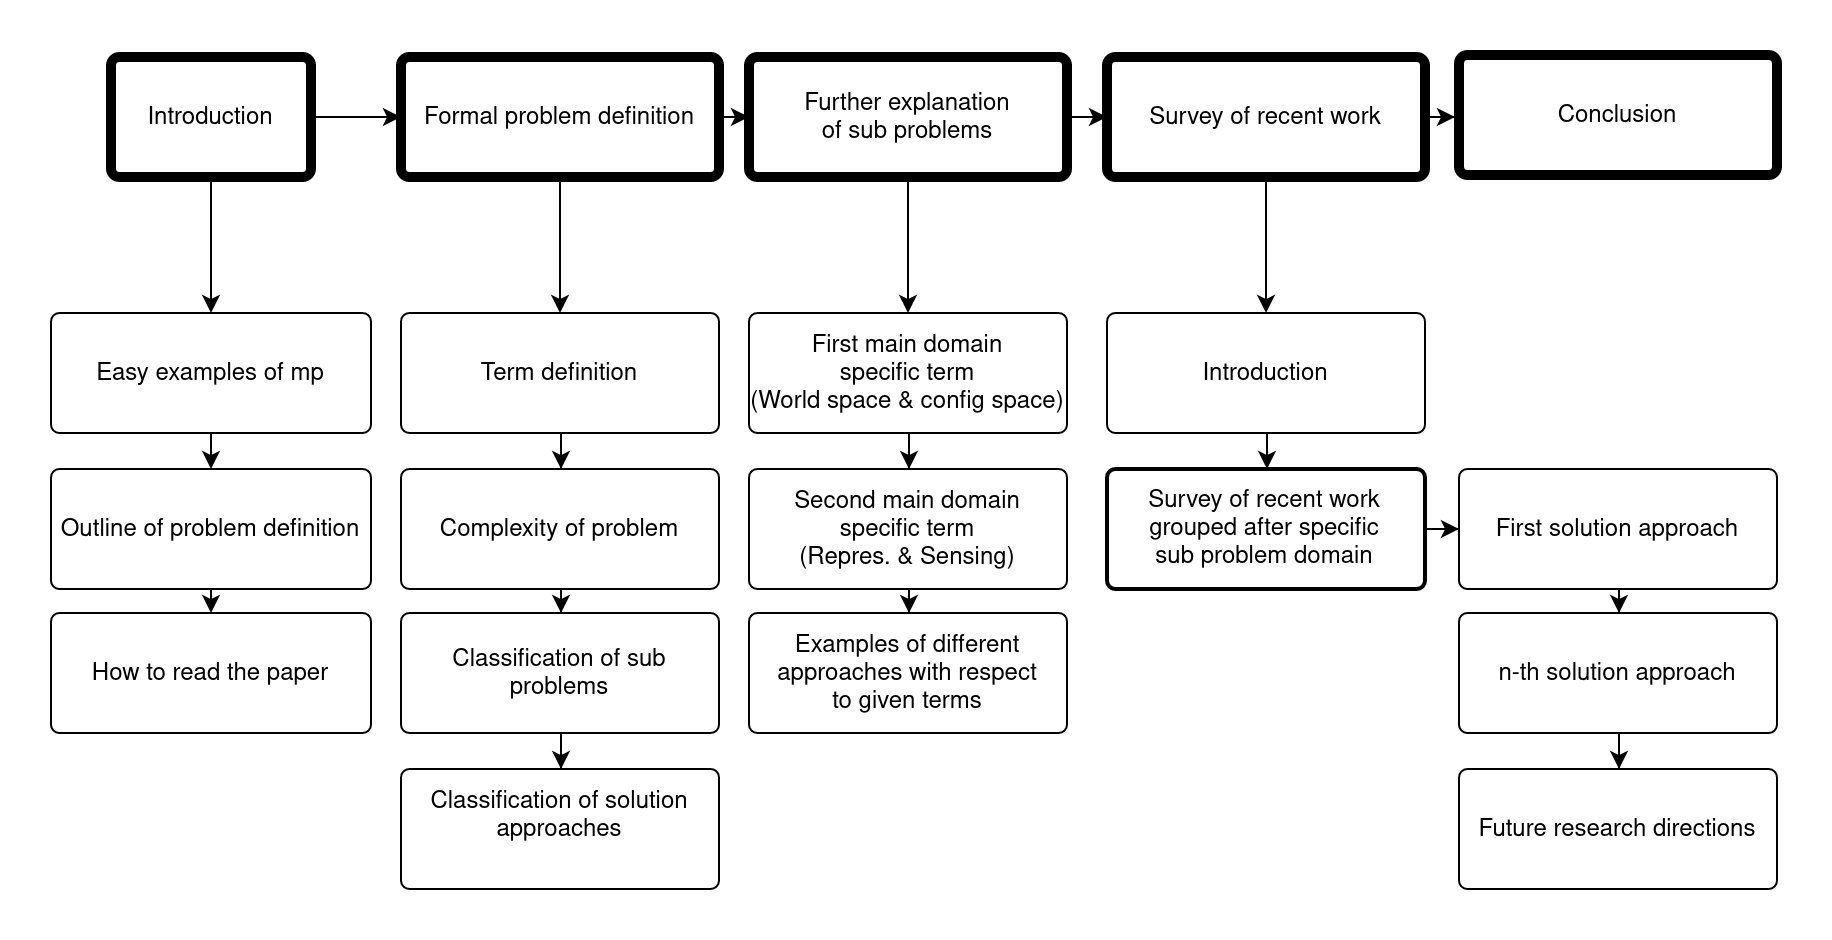
\includegraphics[width=\linewidth]{gmp_flowchart.png}
    \caption{My approach for visualizing the structure}
    \label{fig:nuns}
  \end{figure}


  \section*{Task 3: Special Terms}

  \begin{description}
      \item[glossary] "A list of often difficult or specialized words with their definitions, often placed at the back of a book."\cite{wn_glos:1}
      \item[taxonomy] "An ordered arrangement of groups or categories."\cite{wn_tax:1}
      \item[ontology] "The branch of metaphysics that deals with the nature of being."\cite{wn_onto:1}
  \end{description}
  
  \subsection*{Ontology}
  Why is Ontology the best word:
  \begin{itemize}
      \item Ontology describes the art of creating categories at a very deep level.
      \item Includes taxonomy and glossary
  \end{itemize}

  Description:  "(Computers) A systematic arrangement of all of the important categories of objects or concepts which exist in some field of discourse, showing the relations between them. When complete, an ontology is a categorization of all of the concepts in some field of knowledge, including the objects and all of the properties, relations, and functions needed to define the objects and specify their actions. A simplified ontology may contain only a hierarchical classification (a taxonomy) showing the type subsumption relations between concepts in the field of discourse. An ontology may be visualized as an abstract graph with nodes and labeled arcs representing the objects and relations."\cite{gnu_onto:1}

  \section*{Task 5: Mindmap of the keywords}

  \begin{figure}[h!]
    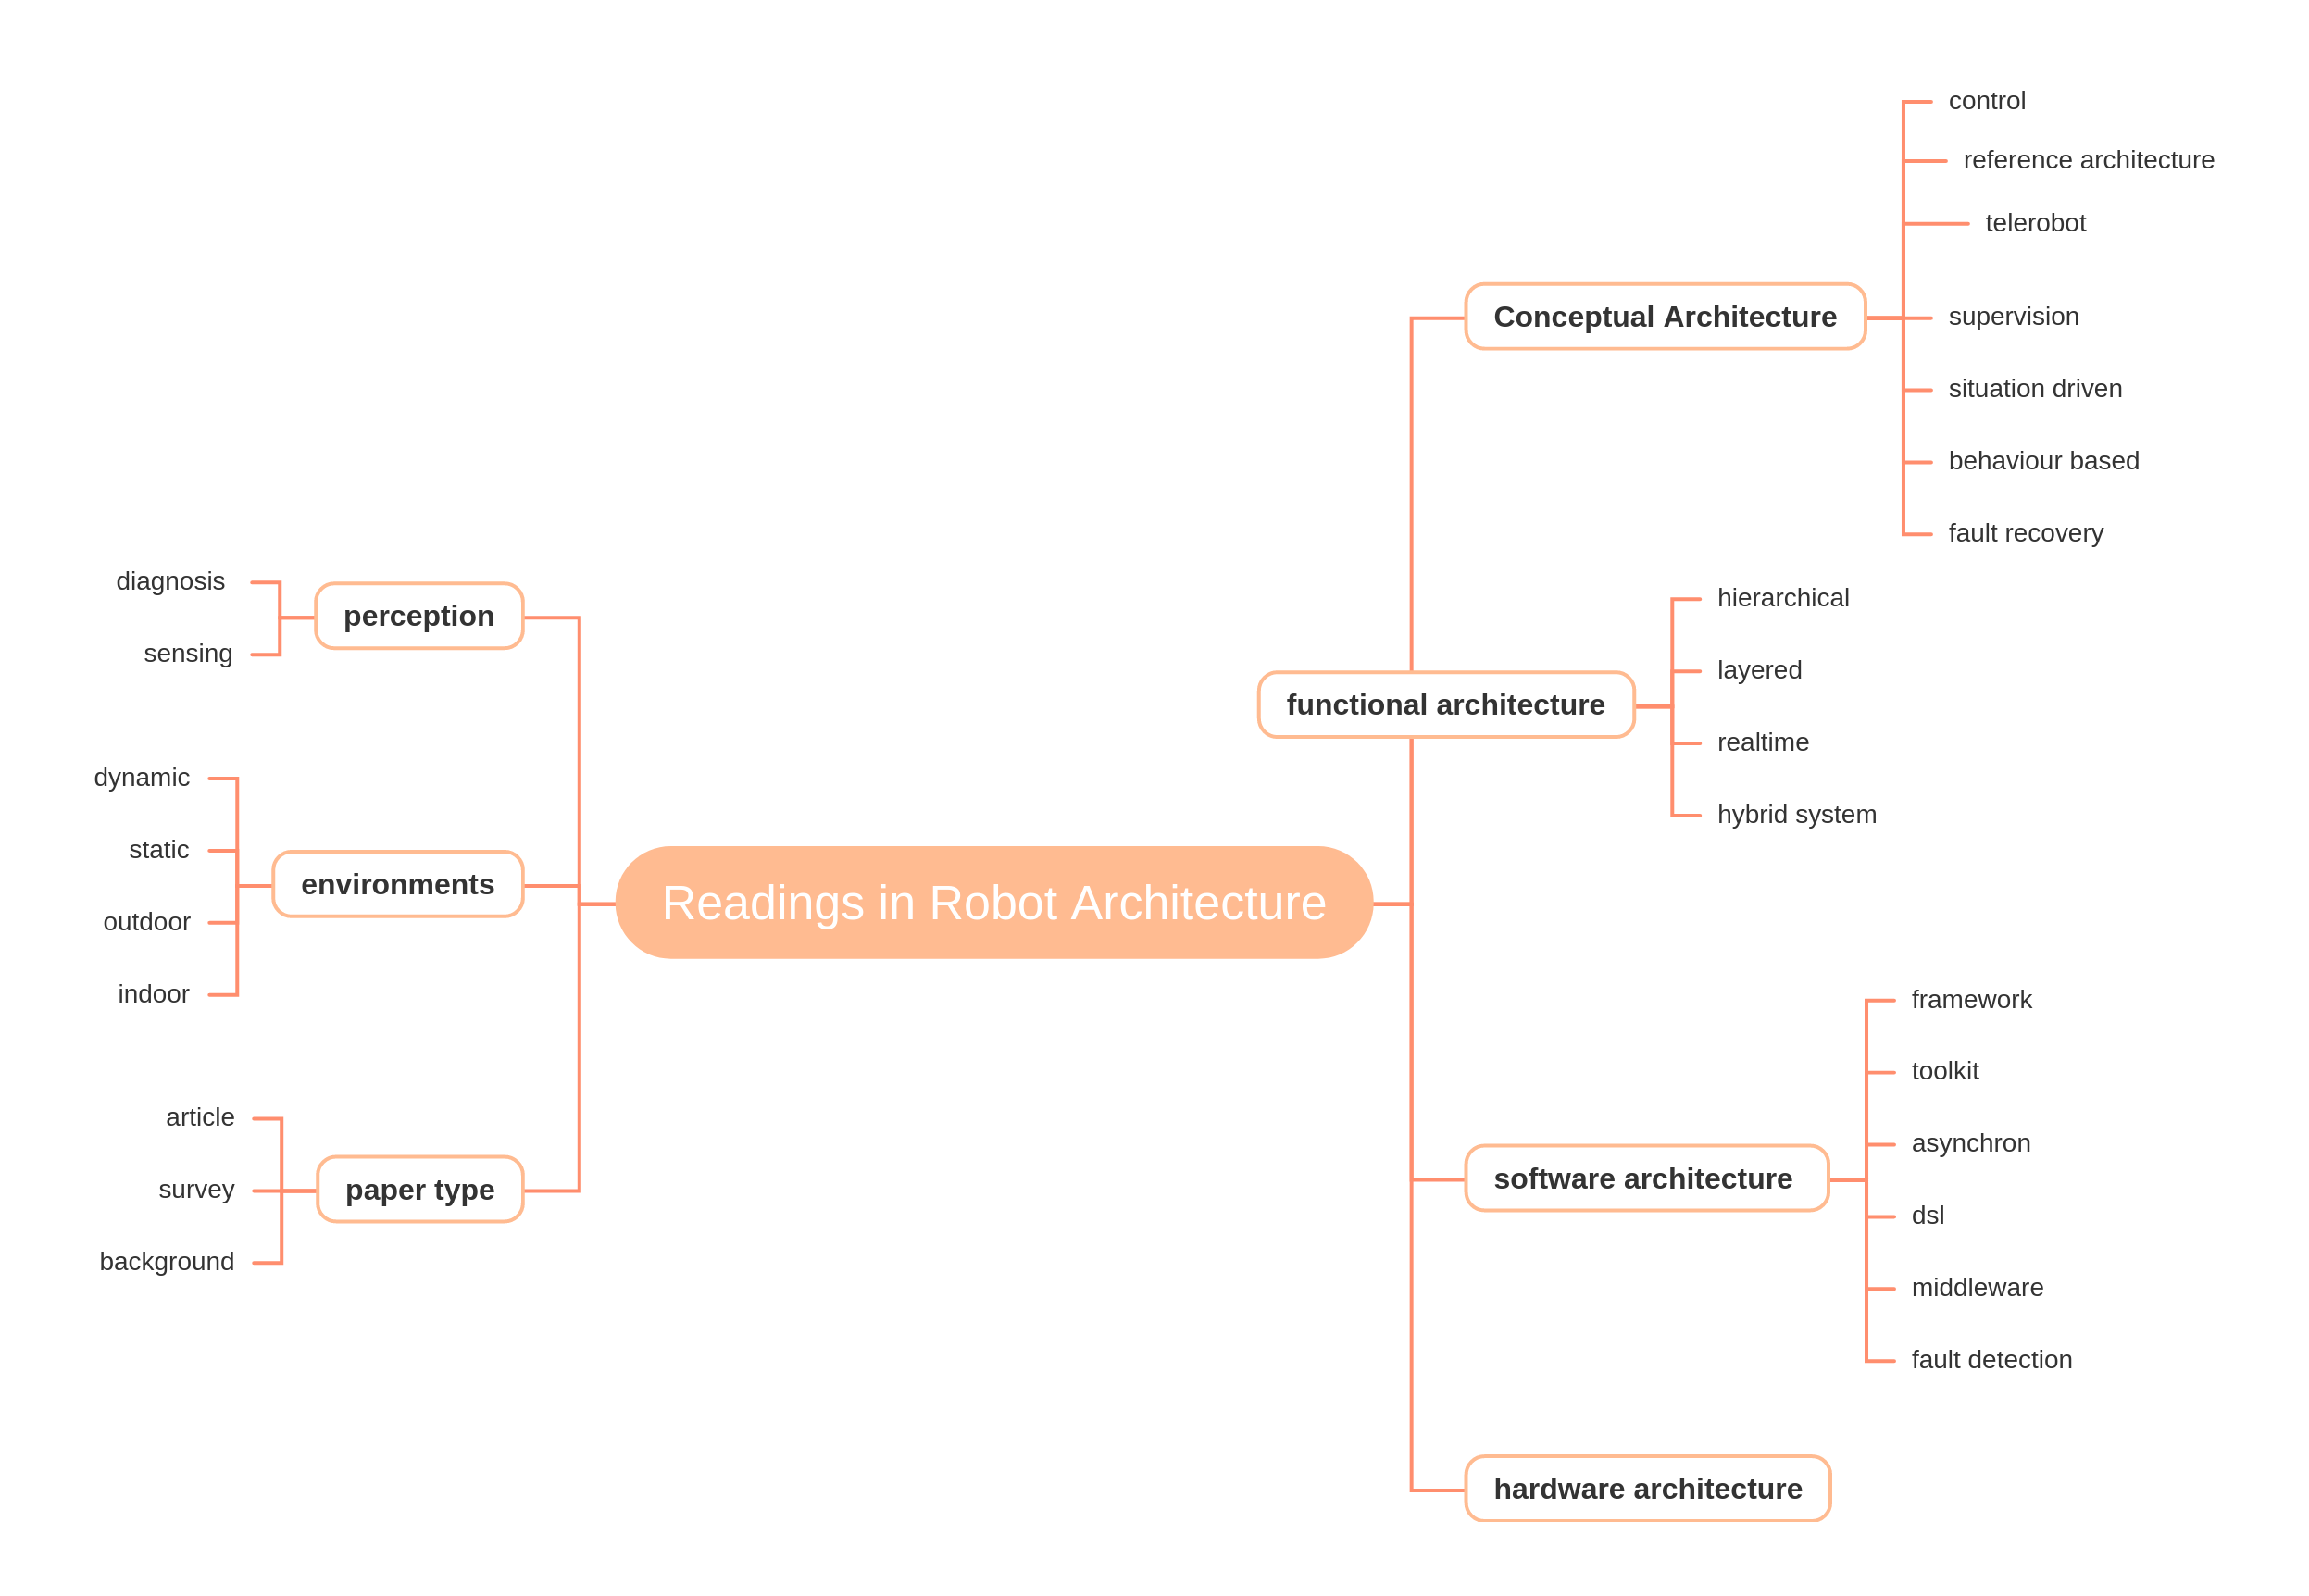
\includegraphics[width=\linewidth]{readings_mm.png}
    \caption{Mindmap over the keywords.}
    \label{fig:nuns}
  \end{figure}

  \break
\bibliography{stuff}
\bibliographystyle{ieeetr}

\end{document}